\documentclass[10pt]{article}
\usepackage{tmlr}
% camera-ready: \usepackage[accepted]{tmlr}; preprint: \usepackage[preprint]{tmlr}

\usepackage{amsmath,amssymb,booktabs,graphicx,xcolor,longtable}
\usepackage{hyperref}
\usepackage{url}
\hypersetup{colorlinks=true,linkcolor=black,citecolor=blue!50!black,urlcolor=blue!50!black}
\usepackage[section]{placeins}

\title{Is the Bayesian OOD Advantage Just Softness?\\Optimizer Time, Mean-Field VI and the Exact Posterior}

\author{\name Anonymous authors\\
      \addr Paper under double-blind review}

\def\month{MM}
\def\year{YYYY}
\def\openreview{\url{https://openreview.net/forum?id=XXXX}}

\begin{document}
\maketitle

\begin{abstract}
Bayesian neural networks are often reported to detect out-of-distribution
(OOD) inputs better than deterministic networks, but their predictions are
also softer everywhere, and softness can be bought with a temperature. We
compare each method with a deterministic network whose temperature is
fitted, on validation data only, to the method's mean in-distribution
entropy. In pre-registered experiments with small MLPs on MNIST-family data,
mean-field Bayes by Backprop (BBB) is no better than this control at standard
budgets on MNIST, but with more optimizer steps it beats it by 0.06--0.08
AUROC, also against step-matched networks and ensembles, weight noise, and
the best temperature chosen with the OOD set. We derive why: under Adam the
KL gradient on the variance parameters is nearly constant, so posterior
standard deviations grow on a learning-rate $\times$ steps clock almost
independent of the data size; under SGD they do not, and no advantage
appears. Under a prior where full-batch HMC converges, the HMC posterior
also beats the control, more than a MAP ensemble under the same prior, and
BBB's mutual information matches its advantage on KMNIST, though by a
structurally different solution. The advantage is a far-OOD effect: on
held-out MNIST classes it disappears.
\end{abstract}

\section{Introduction}
A standard classifier gives confident predictions on inputs unlike its
training data.%
\footnote{Use of AI tools: an LLM-based assistant (Claude, Anthropic) was used
extensively throughout this work: to suggest experiments, analyses and parts
of the derivation in \S\ref{sec:clock}, to draft the pre-registered protocols,
to implement, run and debug the experiment and analysis code, to write and edit
the text, and, as a separate agent, to audit code and claims
(Appendix~\ref{app:hmc}). The authors directed the study, decided what to run
and report, and take full responsibility for all content.} Bayesian neural networks average predictions over a
distribution of weights \citep{blundell2015weight}, which should raise their
uncertainty on unfamiliar inputs, and the usual evidence is that their
predictive entropy separates in-distribution from out-of-distribution (OOD)
inputs better than a deterministic network's.

That evidence has a confound. An averaged prediction is softer than a single
network's on \emph{every} input, and temperature scaling
\citep{guo2017calibration} softens a deterministic network at no cost.
Temperature is a known ingredient of OOD detection
\citep{liang2018enhancing}, uncertainty benchmarks include temperature-scaled
baselines \citep{ovadia2019can}, and \citet{ashukha2020pitfalls} argue that
uncertainty methods should be compared after temperature scaling. Whether
Bayesian posteriors are intrinsically good OOD detectors has also been
questioned \citep{henning2021bayesian}. We make the confound the centre of
the comparison: every method is compared with a deterministic network
softened, on validation data only, to that method's own in-distribution
entropy, and we ask whether the method ranks OOD inputs as more uncertain
than in-distribution inputs better than a network of the same softness.

We study mean-field Bayes by Backprop (BBB), the canonical variational BNN,
on small MLPs where every question can be asked directly, including how the
answer compares with the exact posterior. Every experiment had its
hypotheses, predictions and falsification criteria written down before it
ran; Appendix~\ref{app:ledger} lists all 87 predictions with their outcomes,
31 of which were falsified. Our findings are:
\begin{enumerate}
\item \textbf{The advantage follows optimizer steps.} On MNIST at standard
budgets BBB is no better than the softness-matched network. With more
optimizer steps it beats it by $+0.06$ to $+0.08$ AUROC at every training-set
size we tried, also against step-matched plain networks and deep ensembles,
random weight noise, a plain network at the best temperature chosen with
knowledge of the OOD set, and on correctly classified images only. With
Fashion-MNIST as the in-distribution data the long-training advantage
replicates ($+0.08$ to $+0.21$), but there it is already present at the
standard budget and a step-matched ensemble ties BBB on one OOD set. On a
near-OOD split (trained on digits 0--4, tested against digits 5--9) the
advantage largely disappears ($+0.011$, no better than step-matched
deterministic models), so our claims concern far-OOD detection
(\S\ref{sec:control}).
\item \textbf{An optimizer clock explains when (on MNIST).} Under Adam the gradient of the
KL term on each variance parameter is nearly constant, so the posterior
standard deviations grow by about one learning rate per step, independently of
the data size. This predicts, with no fitted constants, the $1/\eta$ timing
under Adam, its independence of $N$, and the $N$-dependent growth under SGD,
where BBB then shows no advantage. IVON, a natural-gradient method whose
variances scale with $N$, showed none either in our configuration
(\S\ref{sec:clock}).
\item \textbf{The HMC posterior has the advantage too.} Under a prior of
scale 0.3, where full-batch HMC converges (8 chains, three data subsets per
$n$), the posterior beats the softness-matched network by $+0.05$ to $+0.11$.
BBB's mutual information on KMNIST matches it within 0.012; on Fashion-MNIST
and with the entropy score BBB recovers only part of it. Under the default
$\mathcal N(0,1)$ prior HMC does not mix at this scale (\S\ref{sec:hmc}).
\item \textbf{BBB gets there by a different route.} Each weight's marginal
under the exact posterior is the prior, and sampling weights independently
from those marginals gives chance accuracy, as expected for a model with far
more parameters than training points. Long-trained BBB is instead overpruned:
a few precise means carry the prediction. A first-layer noise-to-signal
ratio computed from its means and variances matches its sampled far-OOD
detection within 0.02 AUROC, but on far-OOD sets a trivial pixel statistic
tracks BBB's per-image uncertainty as well, so this is a cheap score rather
than an explanation (\S\ref{sec:route}).
\end{enumerate}
A caveat applies throughout: the standard far-OOD pairs used here are nearly
solved by a model-free rule that flags ink on pixels that are always
background in the training data (AUROC 0.967--1.000). The models do not rely on
it (\S\ref{sec:control}), but it means these benchmarks test a narrow kind of
OOD detection. On a held-out-class split that the rule cannot solve (AUROC
0.57), BBB's advantage largely disappears (\S\ref{sec:control}).

What the paper offers is therefore mainly methodological: a control that
separates a Bayesian method's OOD signal from its softness, evidence that for
mean-field VI that signal depends on the training run rather than the method,
and an account of when it appears. It is not a new OOD detector, and the
effect it studies is confined to far-OOD inputs.

The practical consequence is that a reported OOD gain of a variational BNN is
a property of the training run as much as of the method: comparisons should
report the optimizer, learning rate and budget, the uncertainty score, and a
softness-matched baseline.

\section{Setup}\label{sec:setup}
\paragraph{Data.} In-distribution (ID) data are class-stratified training
subsets of MNIST of size $n\in\{500, 2{,}000, 10{,}000\}$ (one subset per
seed), a fixed validation pool of 5{,}000 further training images, disjoint
from every subset, and the MNIST test set. OOD sets are the Fashion-MNIST
\citep{xiao2017fashion} and KMNIST \citep{clanuwat2018deep} test sets,
normalised with the ID statistics. In Table~\ref{tab:fashion} the roles are
swapped: Fashion-MNIST is ID, MNIST and KMNIST are OOD; and in a held-out-class
split, the network is trained on digits 0--4 and the test digits 5--9 are a
near-OOD set.

\paragraph{Models.} All models use a 784--256--256--10 ReLU MLP (width 100
for the HMC comparison). \emph{DNN}: Adam ($10^{-3}$, cosine schedule), 40
epochs, batch 64. \emph{Deep ensemble} \citep{lakshminarayanan2017simple}: 5
DNNs. \emph{MC dropout} \citep{gal2016dropout}: $p=0.1$, 50 samples.
\emph{Last-layer Laplace} \citep{daxberger2021laplace}: full generalised
Gauss--Newton covariance over the last layer, prior precision tuned on
validation NLL. \emph{IVON} \citep{shen2024variational}: the official
implementation with effective sample size $N$ and the same $\mathcal N(0,1)$
prior as BBB. \emph{BBB} \citep{blundell2015weight}: mean-field Gaussian
posterior, $\mathcal N(0,\sigma_p^2)$ prior with $\sigma_p=1$ unless stated,
and per-example negative ELBO
\begin{equation}
\mathcal{L} = \frac{1}{B}\sum_{i\in\text{batch}} -\log p(y_i\mid x_i, w)
+ \frac{1}{N}\,\mathrm{KL}\big[q(w)\,\|\,p(w)\big], \qquad w=\mu+\sigma\odot\varepsilon,
\label{eq:elbo}
\end{equation}
with the KL weight warmed up linearly, $\sigma=\mathrm{softplus}(\rho)$,
$\rho_0=-5$ ($\sigma_0\approx0.007$), Adam ($10^{-3}$), gradient clipping and
50 posterior samples at test time. The standard budget is 150 epochs at
$n\ge2{,}000$ (4{,}800 steps at $n=2{,}000$, 23{,}550 at $n=10{,}000$) and the same
4{,}800 steps at $n=500$ (600 epochs). Dividing the KL
term by the number of mini-batches instead of $N$, an easy slip, over-weights
it by about the batch size and costs 3 points of accuracy
(Appendix~\ref{app:kl}).

\paragraph{The softness-matched control.} For a method $M$ we fit a
temperature $T$ to a DNN's logits so that its mean predictive entropy on the
validation set equals $M$'s; no test or OOD data enter the fit. We report
\begin{equation}
\Delta=\mathrm{AUROC}(M)-\mathrm{AUROC}(\mathrm{DNN}_T),
\end{equation}
where AUROC measures the separation of test from OOD images by predictive
entropy; $\Delta>0$ means $M$ ranks OOD inputs better than a network of the
same mean softness; the shape of the entropy distribution is not matched. The
MI-based $\Delta$ uses $M$'s mutual information
\citep{depeweg2018decomposition} instead, against the same softened network's
entropy. A single network has no mutual information, so this compares two
different scores: it asks whether $M$'s epistemic score beats the best
softness-based score of a plain network. It is only meaningful for a model
that has learned the task, since a model whose posterior samples disagree on
every input also has a large MI-based $\Delta$ (\S\ref{sec:clock}). Comparisons are
paired by seed with bootstrap confidence intervals and sign counts; Wilcoxon
tests are reported only with 10 seeds.

\paragraph{Pre-registration.} Each experiment's protocol (hypothesis,
predictions, falsification criterion, configuration) was written before it
ran: committed to version control for the first nine experiments and, for
the rest, with a SHA-256 hash of the protocol recorded before launch. These
records are self-attested rather than independently timestamped. Experiments
are referred to by their identifiers (E1--E23); Appendix~\ref{app:ledger}
lists every prediction.

\section{The advantage follows optimizer steps}\label{sec:control}
\paragraph{At standard budgets, BBB matches the control.} Table~\ref{tab:grid}
compares each method with its own softness-matched DNN over 10 seeds (E2).
At $n=500$ and $n=2{,}000$, BBB is \emph{worse} than the control (0/10 seeds
better on KMNIST at both, 0/10 and 3/10 on Fashion-MNIST). At $n=10{,}000$ it is
better in all 10 seeds. Deep ensembles beat the control by $+0.01$ to $+0.02$
at every $n$, MC dropout roughly ties it, and last-layer Laplace is below it.

\begin{table}[!htb]
\centering\small
\caption{Each method against a DNN softened to its own validation entropy
(entropy-AUROC difference $\Delta$, mean and 95\% bootstrap CI over 10 seeds;
standard budgets; E2).}
\label{tab:grid}
\begin{tabular}{llcc}
\toprule
$n$ & method & $\Delta$ Fashion-MNIST & $\Delta$ KMNIST \\
\midrule
500 & BBB & $-0.046$ [$-0.063$, $-0.032$] & $-0.035$ [$-0.041$, $-0.028$] \\
500 & ensemble & $+0.014$ [$0.003$, $0.027$] & $+0.010$ [$0.008$, $0.012$] \\
500 & MC dropout & $-0.003$ [$-0.016$, $0.009$] & $-0.019$ [$-0.021$, $-0.018$] \\
500 & last-layer Laplace & $-0.072$ [$-0.088$, $-0.055$] & $-0.112$ [$-0.122$, $-0.102$] \\
\midrule
2{,}000 & BBB & $-0.024$ [$-0.048$, $-0.001$] & $-0.010$ [$-0.014$, $-0.007$] \\
2{,}000 & ensemble & $+0.015$ [$0.007$, $0.022$] & $+0.015$ [$0.013$, $0.018$] \\
2{,}000 & MC dropout & $+0.007$ [$0.002$, $0.012$] & $-0.010$ [$-0.012$, $-0.007$] \\
2{,}000 & last-layer Laplace & $-0.040$ [$-0.047$, $-0.032$] & $-0.043$ [$-0.047$, $-0.038$] \\
\midrule
10{,}000 & BBB & $\mathbf{+0.048}$ [$0.038$, $0.059$] & $\mathbf{+0.069}$ [$0.065$, $0.074$] \\
10{,}000 & ensemble & $+0.016$ [$0.008$, $0.026$] & $+0.023$ [$0.021$, $0.025$] \\
10{,}000 & MC dropout & $-0.010$ [$-0.018$, $-0.001$] & $-0.007$ [$-0.010$, $-0.003$] \\
10{,}000 & last-layer Laplace & $-0.014$ [$-0.023$, $-0.006$] & $-0.012$ [$-0.016$, $-0.008$] \\
\bottomrule
\end{tabular}
\end{table}

\paragraph{The jump at $n=10{,}000$ is about steps, not data.} With a fixed
number of epochs, more data also means more optimizer steps (23{,}550 at
$n=10{,}000$ against 4{,}800). Decoupling the two (E4,
Figure~\ref{fig:steps}): with the same data, 23{,}550 steps give
$\Delta=+0.06$ to $+0.08$ in 5/5 seeds at every $n$, including $n=500$, while
4{,}800 steps give a negligible one at most, including at $n=10{,}000$ ($-0.006$
on Fashion-MNIST, $+0.008$ on KMNIST).

\begin{figure}[!htb]
\centering
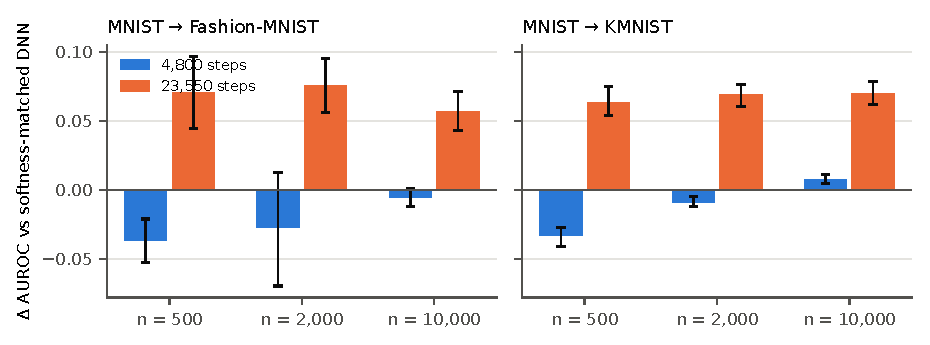
\includegraphics[width=0.85\linewidth]{../figures/paper_steps_vs_n.pdf}
\caption{BBB against its softness-matched DNN with the same training data and
two step budgets (5 seeds, 95\% CIs; E4).}
\label{fig:steps}
\end{figure}

\paragraph{Stronger controls do not close the gap.} Long-trained BBB
(23{,}550 steps) also beats controls that share its training budget or its
noise (E12, Table~\ref{tab:controls}; 5 seeds, $n\in\{2{,}000,10{,}000\}$). A plain
network and a 5-member ensemble trained for the same number of steps stay
below it in all 5 seeds in every setting. Adding Gaussian noise to every layer
of a trained plain network, scaled per layer and matched to BBB's validation
entropy, gives AUROC 0.81--0.89, and BBB beats it by $+0.10$ to $+0.15$; even
the best noise scale chosen with knowledge of the OOD set stays $+0.07$ to
$+0.10$ below BBB. So the advantage is not produced by \emph{any} weight noise.
Among post-hoc deterministic detectors, a kNN detector on normalised
penultimate features comes closest (within $+0.006$ to $+0.023$, and tying BBB
at $n=10{,}000$ on Fashion-MNIST, 2/5 seeds better).

\begin{table}[!htb]
\centering\small
\caption{Long-trained BBB (23{,}550 steps) minus each control (entropy AUROC;
range over $n\in\{2{,}000,10{,}000\}$ and, for feature detectors, two base
networks; 5 seeds each; E12).}
\label{tab:controls}
\begin{tabular}{lcc}
\toprule
control & Fashion-MNIST & KMNIST \\
\midrule
plain network + weight noise (softness-matched) & $+0.11$ to $+0.14$ & $+0.10$ to $+0.15$ \\
step-matched plain network, softened & $+0.040$ to $+0.087$ & $+0.075$ to $+0.078$ \\
step-matched 5-member ensemble & $+0.041$ to $+0.058$ & $+0.058$ to $+0.075$ \\
Mahalanobis on features & $+0.021$ to $+0.109$ & $+0.030$ to $+0.059$ \\
kNN on features & $+0.006$ to $+0.023$ & $+0.017$ to $+0.023$ \\
\bottomrule
\end{tabular}
\end{table}

\paragraph{Softness matters, but does not explain the advantage.} Is the
softness-matched control a strawman? A post-hoc sweep over temperatures
(exploratory; Table~\ref{tab:sweep}) shows that it is not: temperature moves the
plain network's entropy AUROC by about 0.10 between the worst and best
temperature on a grid from 0.25 to 50, and the best temperature, chosen
\emph{with} knowledge of the OOD set, gains $+0.035$ over $T=1$ on average. But
long-trained BBB beats even this oracle-tempered network in every seed of every
setting (50/50; by $+0.042$ to $+0.070$ with MNIST as ID and $+0.079$ to $+0.196$
with Fashion-MNIST). Nor is the advantage a side effect of BBB being uncertain
on misclassified in-distribution images: restricted to test images that both
BBB and the plain network classify correctly, $\Delta$ stays positive in every
setting ($+0.046$ to $+0.062$ on MNIST, $+0.053$ to $+0.175$ on Fashion-MNIST).
With the cosine schedule used here, long-trained BBB on MNIST is as accurate as
the plain network (0.933 against 0.925 at $n=2{,}000$); on Fashion-MNIST it is
less accurate (0.762 against 0.827).

\begin{table}[!htb]
\centering\small
\caption{How much can temperature buy? Entropy AUROC of long-trained BBB and of
the plain 40-epoch network at $T=1$, at the softness-matched $T$, and at the
best $T$ on a log grid from 0.25 to 50 chosen with the OOD set (oracle); last
column: $\Delta$ on test images both classify correctly. Means over 5 seeds
(post-hoc, exploratory).}
\label{tab:sweep}
\begin{tabular}{lllccccc}
\toprule
ID & $n$ & OOD & BBB & DNN, $T=1$ & DNN, matched $T$ & DNN, oracle $T$ & $\Delta$ (both correct) \\
\midrule
MNIST & 500 & Fashion & 0.907 & 0.813 & 0.837 & 0.860 & $+0.058$ \\
MNIST & 500 & KMNIST & 0.955 & 0.852 & 0.891 & 0.913 & $+0.046$ \\
MNIST & 2{,}000 & Fashion & 0.951 & 0.862 & 0.875 & 0.888 & $+0.062$ \\
MNIST & 2{,}000 & KMNIST & 0.968 & 0.871 & 0.899 & 0.909 & $+0.055$ \\
MNIST & 10{,}000 & Fashion & 0.973 & 0.904 & 0.916 & 0.917 & $+0.050$ \\
MNIST & 10{,}000 & KMNIST & 0.987 & 0.903 & 0.917 & 0.918 & $+0.058$ \\
Fashion & 2{,}000 & MNIST & 0.980 & 0.779 & 0.844 & 0.845 & $+0.082$ \\
Fashion & 2{,}000 & KMNIST & 0.827 & 0.716 & 0.745 & 0.747 & $+0.053$ \\
Fashion & 10{,}000 & MNIST & 0.956 & 0.756 & 0.796 & 0.797 & $+0.117$ \\
Fashion & 10{,}000 & KMNIST & 0.885 & 0.682 & 0.678 & 0.689 & $+0.175$ \\
\bottomrule
\end{tabular}
\end{table}

\paragraph{Not a pixel shortcut.} MNIST subsets have many always-background
pixels, and a model-free rule that flags ink on such pixels separates MNIST
from Fashion-MNIST and KMNIST almost perfectly (AUROC 0.967--1.000), better
than any model here, a real weakness of these benchmarks. The models do not rely on it: resetting those
pixels to background in the OOD images leaves every method's $\Delta$
essentially unchanged (E5, Appendix~\ref{app:pixels}). The advantage also needs
posterior noise in both hidden layers together; noise in any single layer
keeps essentially none of it (E6b, Appendix~\ref{app:layers}).

\paragraph{With Fashion-MNIST as the in-distribution data.}\label{sec:fashion}
To test whether these results are specific to MNIST, we swapped the roles
(E21; Fashion-MNIST as ID, MNIST and KMNIST as OOD; 5 seeds;
Table~\ref{tab:fashion}). The long-training result replicates and is larger:
BBB trained for 23{,}550 steps beats the softness-matched network by $+0.136$
(MNIST) and $+0.082$ (KMNIST) at $n=2{,}000$, and by $+0.160$ and $+0.206$ at
$n=10{,}000$, in 5/5 seeds, and it beats the step-matched plain network in 5/5
seeds on both OOD sets. Three predictions failed or held only in part. First,
BBB already beats the control at the standard budget ($+0.080$ and $+0.066$),
so the absence of an advantage at standard budgets in Table~\ref{tab:grid} is
specific to MNIST; one reading is that the clock of \S\ref{sec:clock} fixes
\emph{when} the variances grow, not how much variance a dataset needs before
the advantage appears. Second, the step-matched ensemble ties BBB on KMNIST
($\Delta$ $+0.084$ against $+0.082$; BBB higher in 2/5 seeds), although BBB's
absolute entropy AUROC is higher (0.827 against 0.792). Third, long-trained
BBB's MI-based $\Delta$ on MNIST is only $+0.015$. Long training also costs 6.5
points of accuracy here (0.762 against 0.827), and plain networks are much
weaker detectors with Fashion-MNIST as ID (entropy AUROC 0.68--0.84), so even
step-matched deterministic training gains a little ($+0.018$ to $+0.040$).

\begin{table}[!htb]
\centering\small
\caption{Fashion-MNIST as in-distribution data, MNIST and KMNIST as OOD:
$\Delta$ against the softness-matched 40-epoch DNN (mean over 5 seeds, seeds
with $\Delta>0$ in brackets; E21).}
\label{tab:fashion}
\begin{tabular}{llcccc}
\toprule
$n$ & method & acc. & $\Delta$ MNIST & $\Delta$ KMNIST & MI $\Delta$ MNIST / KMNIST \\
\midrule
2{,}000 & DNN (reference) & 0.827 & & & \\
2{,}000 & BBB, standard (4{,}800 steps) & 0.831 & $+0.080$ (5/5) & $+0.066$ (5/5) & $+0.105$ / $+0.109$ \\
2{,}000 & BBB, 23{,}550 steps & 0.762 & $+0.136$ (5/5) & $+0.082$ (5/5) & $+0.015$ / $+0.205$ \\
2{,}000 & DNN, 23{,}550 steps & 0.823 & $+0.040$ (5/5) & $+0.018$ (5/5) & \\
2{,}000 & ensemble, 40 epochs & 0.829 & $+0.038$ (5/5) & $+0.043$ (5/5) & $+0.099$ / $+0.112$ \\
2{,}000 & ensemble, 23{,}550 steps & 0.827 & $+0.085$ (5/5) & $+0.084$ (5/5) & $+0.092$ / $+0.094$ \\
\midrule
10{,}000 & DNN (reference) & 0.863 & & & \\
10{,}000 & BBB, standard (23{,}550 steps) & 0.849 & $+0.160$ (5/5) & $+0.206$ (5/5) & $+0.180$ / $+0.295$ \\
\bottomrule
\end{tabular}
\end{table}

\paragraph{Held-out classes: the advantage is a far-OOD effect.}\label{sec:near}
A pre-registered held-out-class split (E22; 5 seeds) trains on MNIST digits 0--4
($n=2{,}000$) and treats the test digits 5--9 as OOD, with Fashion-MNIST and
KMNIST for reference. Here the pixel rule is close to chance (AUROC 0.569,
against 1.000 and 0.999 on the far-OOD sets), so a detector must use more than
where the ink is. The plain network reaches 0.890 on held-out digits. Long-trained
BBB's advantage over its softness-matched network is only $+0.011$ (4/5 seeds),
below our pre-registered threshold of $+0.02$, and no larger than that of a
step-matched plain network ($+0.010$; BBB higher in 3/5 seeds) or a step-matched
ensemble ($+0.018$; BBB higher in 1/5); standard-budget BBB does slightly better
($+0.023$). On the far-OOD sets of the same models long-trained BBB keeps an
advantage ($+0.047$ and $+0.034$), though smaller than in the ten-class setting
of Table~\ref{tab:grid} and Figure~\ref{fig:steps}. This is consistent with the
mechanism in \S\ref{sec:route}, which locates BBB's OOD signal in how inputs
drive its first layer and which fails for near-OOD rotated digits, but we did
not test the first-layer account on this split. The results in this paper
therefore concern far-OOD detection.

\section{An optimizer clock}\label{sec:clock}
\paragraph{Derivation.} For one weight with posterior $\mathcal N(\mu,\sigma^2)$
and prior $\mathcal N(0,\sigma_p^2)$,
\begin{equation}
\mathrm{KL}=\log\frac{\sigma_p}{\sigma}+\frac{\sigma^2+\mu^2}{2\sigma_p^2}-\frac12,
\qquad
\frac{\partial\,\mathrm{KL}}{\partial\rho}
=\Big(\frac{\sigma}{\sigma_p^2}-\frac{1}{\sigma}\Big)\,\mathrm{sigmoid}(\rho)
\;\approx\;-1 \quad\text{for } \rho\ll 0,
\label{eq:klgrad}
\end{equation}
because $\sigma=\mathrm{softplus}(\rho)\approx\mathrm{sigmoid}(\rho)\approx e^{\rho}$
when $\rho\ll0$. In Eq.~\ref{eq:elbo} this gradient is weighted by $1/N$,
and while $\sigma$ is small the likelihood term's gradient on $\rho$, which
scales with $\sigma$, is negligible; the gradient on each $\rho$ is then
roughly the constant $-1/N$. Adam divides each gradient by a running estimate
of its magnitude, so a gradient of constant sign produces a step of about the
learning rate $\eta$, independently of its size and hence of $N$ (Adam's
sign-descent behaviour, \citealp{balles2018dissecting}). The number of steps
for $\rho$ to travel from $\rho_0$ to $\rho^\star$ is therefore
\begin{equation}
t^\star \approx \frac{\rho^\star-\rho_0}{\eta}.
\label{eq:clock}
\end{equation}
For $\sigma=0.3$ ($\rho^\star=-1.05$) from $\rho_0=-5$ this gives
$t^\star\approx 3{,}950$ steps at $\eta=10^{-3}$. Under SGD with momentum $\beta$
the step is instead $\eta_\rho/(N(1-\beta))$, so the same growth takes $N$
times longer as $N$ grows. The approximation fails once $\sigma$ is no longer
small compared with the prior, or once the likelihood pulls back.
\citet{unlu2020variational} observe that mean-field variance parameters are
often unconverged when training stops, and \citet{nishida2022adamb} report
that BBB's variational parameters grow under Adam; Eq.~\ref{eq:clock} makes
that growth quantitative and links it to OOD detection.

\paragraph{Test under Adam.} We trained BBB with a constant learning rate for
40{,}000 steps at three learning rates and $n\in\{500,10{,}000\}$ (E10, 3 seeds per
arm; Figure~\ref{fig:clock}, left). The time for the mean first-layer $\sigma$ to
reach 0.3 was 10{,}000, 5{,}000 and 3{,}000 steps at $n=500$ and 12{,}000,
6{,}000 and 3{,}000 at $n=10{,}000$ for $\eta=5\times10^{-4}$, $10^{-3}$ and
$2\times10^{-3}$ (checkpoints every 1{,}000 steps, so the fastest arm is resolved
only to about $\pm$1{,}000 steps): time $\times$ learning rate was constant to
within the checkpoint resolution, and a twenty-fold change in $n$ changed it by
at most 20\%. Eq.~\ref{eq:clock}
predicts 7{,}900, 3{,}950 and 1{,}975 steps with no fitted constant. It gets the
$1/\eta$ scaling and the independence from $n$ right; the observed times are
1.27--1.52 times longer, consistent with gradient noise shrinking Adam's
steps, and the gap is larger at $n=10{,}000$, where the constant $1/N$ signal
is weaker relative to the mini-batch noise. The onset of the OOD advantage
roughly followed the same clock: onset $\times$ learning rate (in units of
$10^3$ steps $\times 10^{-3}$) was 5.5, 5.3 and 6.0 at $n=10{,}000$, but 6.5, 7.7 and
10 at $n=500$, where the largest learning rate later collapsed training (final
accuracy 0.32).

\paragraph{Test under SGD.} With SGD (momentum 0.9) on the $\rho$ parameters,
the mean $\sigma$ after 20{,}000 steps was 0.67 at $n=500$ and 0.017 at
$n=10{,}000$, a 39-fold difference (Figure~\ref{fig:clock}, right). In the
latter setting $\sigma$ never grew, and BBB had \emph{no} OOD advantage (peak
$\Delta$ $-0.007$) while reaching the best accuracy of all runs (0.966). With
gradient clipping restricted to the means (E13), the SGD form of
Eq.~\ref{eq:clock} predicts the numbers with no fitted constant: with
$\eta_\rho=0.05$ the step on $\rho$ is about $5\times10^{-5}$ at $n=10{,}000$,
giving $\sigma\approx0.018$ after 20{,}000 steps against 0.0177 observed, and
$10^{-3}$ at $n=500$, giving $\sigma=0.3$ after about 4{,}300 steps, against a
first checkpoint above 0.3 at 5{,}000. The same optimizer then gives opposite
OOD outcomes depending on whether $\sigma$ grows: at $n=500$, where it does, BBB
reaches an advantage of $+0.057$ to $+0.060$ without clipping; at $n=10{,}000$,
where it does not, there is none. This within-optimizer contrast is the most
direct causal evidence we have that the variance growth, not the optimizer
or the data size as such, switches the advantage on. Unclipped SGD on $\rho$
was unstable once $\sigma$ grew large (6 of 9 runs diverged), which limits what
the SGD arm can show beyond the growth phase (Appendix~\ref{app:ledger}).

\begin{figure}[!htb]
\centering
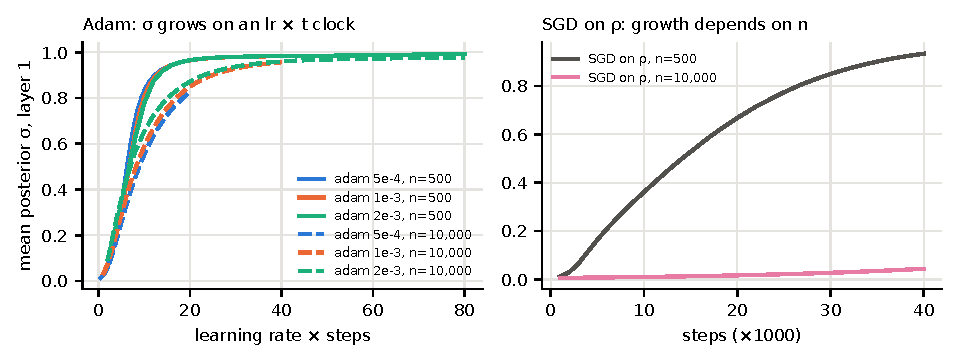
\includegraphics[width=0.85\linewidth]{../figures/E10_clock.pdf}
\caption{Mean first-layer posterior $\sigma$ (mean of 3 seeds; E10). Left: Adam at
three learning rates and two training-set sizes, against learning rate
$\times$ steps. Right: SGD on the $\rho$ parameters, against steps.}
\label{fig:clock}
\end{figure}

\paragraph{Natural-gradient VI escapes the clock, and showed no advantage.}
IVON keeps a Gaussian posterior $\mathcal N(m, 1/(N(h+\delta)))$ whose variance
is set by $N$ and a running curvature estimate $h$, not by a step count. In
a pre-registered comparison (E14; 3 seeds per $n$, 40{,}000 steps), its mean
first-layer $\sigma$ was 0.170, 0.086 and 0.039 at $n=500$, $2{,}000$ and
$10{,}000$; the ratio of 4.41 between the extremes is close to the $1/\sqrt N$
value of 4.47, and the variances stayed far below the prior instead of
drifting to it as BBB's did (0.96--0.98). At $n\ge2{,}000$ IVON was as accurate
as the plain network, but it had no advantage over the softness-matched
network (peak $\Delta$ $-0.005$ and $-0.008$, against BBB's $+0.07$ and $+0.065$), in
the one configuration we ran (learning rate and initial Hessian chosen once by
validation NLL).
Inflating its variances 3.1--9.3$\times$ by tempering the likelihood did not
create one (E15, Appendix~\ref{app:ledger}).

\paragraph{Along training: entropy and mutual information diverge.} Under the
$\mathcal N(0,1)$ prior the clock keeps running past the useful range
(E6, Figure~\ref{fig:dyn}). At $n=2{,}000$ with a constant learning rate, the
entropy-based $\Delta$ on KMNIST peaks at $+0.067$ to $+0.074$ around
9{,}000--14{,}000 steps and is negative again by 25{,}000--30{,}000, as the model
also becomes uncertain on in-distribution digits (mean test entropy rises
from 0.30 to 0.94 as accuracy falls from 0.93 to 0.89), while the negative
ELBO keeps improving. The MI-based $\Delta$ does not fall ($+0.071$ at 30{,}000
steps, $+0.061$ at 50{,}000). This drift is the posterior moving to an
oversized prior: with $\sigma_p=0.3$ (E11), $\sigma$ plateaus at the prior scale
by about 10{,}000 steps and both advantages persist (entropy $\Delta$ $+0.045$
and $+0.048$ at 40{,}000 steps, against $-0.009$ and $+0.015$ for
$\sigma_p=1$). Two cautions follow. A positive MI-based $\Delta$ does not by
itself indicate a useful model: runs initialised with $\sigma_0\ge0.31$ never
learn (chance accuracy) yet have the largest MI-based $\Delta$ (about
$+0.10$). And neither held-out NLL nor the ELBO picks a good stopping point;
a fixed step count does as well as a synthetic-outlier selection rule
(E9, Appendix~\ref{app:stop}), as the clock suggests.

\begin{figure}[!htb]
\centering
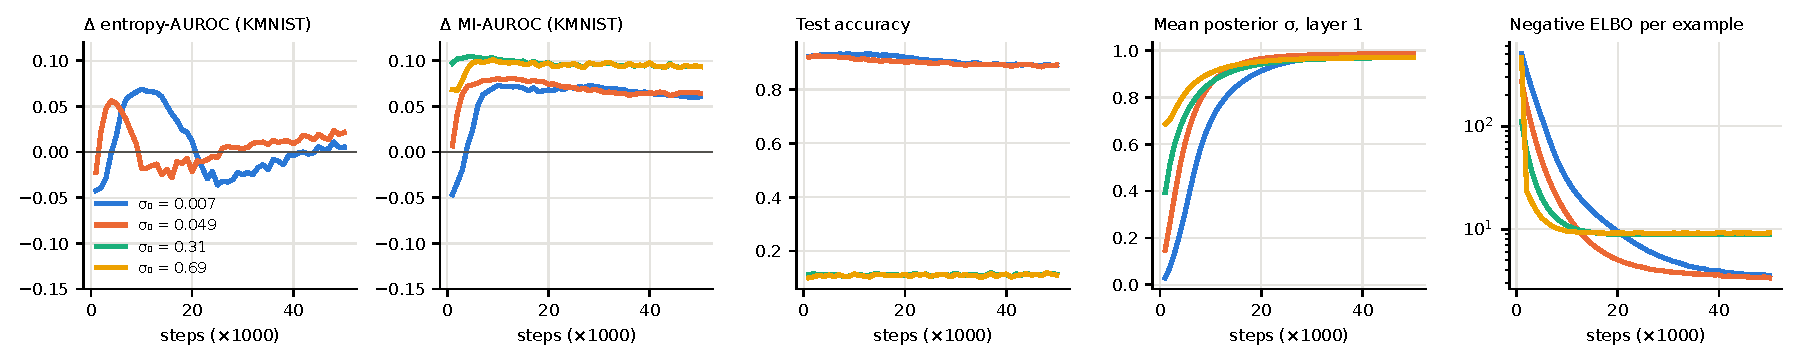
\includegraphics[width=\linewidth]{../figures/E6_dynamics.pdf}
\caption{BBB training dynamics at $n=2{,}000$ (constant learning rate; mean of
3 seeds per initial $\sigma_0$; 20 posterior samples; E6). Runs with
$\sigma_0\ge0.31$ never learn; their entropy-based $\Delta$ (about $-0.86$) is below
the plotted range.}
\label{fig:dyn}
\end{figure}

\section{The exact posterior}\label{sec:hmc}
Is the advantage a property of the Bayesian posterior, or of mean-field VI
under Adam? We compared BBB with full-batch Hamiltonian Monte Carlo
\citep{neal2011mcmc} on the same model at width 100 (89{,}610 parameters),
$n\in\{500,2{,}000\}$. ``Exact posterior'' below means the posterior that HMC
samples, as estimated from 800 samples per run with convergence checked on
predictions, not on weights (which weight-space symmetries make
uninformative). The softness-matched network here is the plain width-100 DNN,
trained without a prior.

\paragraph{Under $\mathcal N(0,1)$, HMC does not mix at this scale.} With 4
chains of 2{,}500 iterations (E19), split-$\hat R$ on the predicted probability
of the true class had a 90th percentile of 2.8 and 2.5 (threshold 1.1), so we
draw no conclusion from that run. The obstacle is the posterior: its weights
sit near the prior scale (standard deviation $\approx0.85$ in every layer),
the logits reach $\sim$700, and the likelihood acts like a hard wall around
``every training point correct''. The stable leapfrog step fell from
$\sim3\times10^{-5}$ at 300-step trajectories to $\sim1.5\times10^{-6}$ at
$10^4$ steps; a diagonal mass matrix and a narrower network did not help
(pilots that looked only at sampler diagnostics; Appendix~\ref{app:hmc}).

\paragraph{Under $\mathcal N(0,0.3^2)$ it converges, and the exact posterior has
the advantage.} A prior of scale 0.3 is where BBB's advantage is stable
(\S\ref{sec:clock}). There the median stable step size was about 20--30
times larger at similar trajectory lengths. Eight chains per run (E20, E20b;
identity mass matrix; dual-averaging step size \citep{hoffman2014nuts};
trajectory length $\pi\sigma_p/2$ \citep{izmailov2021what}; 500 warm-up and
1{,}000 sampling iterations, 100 kept samples per chain) passed the
convergence check in all six runs (two values of $n$, three data subsets;
90th-percentile $\hat R$ 1.004--1.005, maximum 1.022). BBB was retrained under
the same prior for 23{,}550 steps. The exact posterior beats the
softness-matched network on both OOD sets on every run ($\Delta_K$ $+0.052$
to $+0.077$, $\Delta_F$ $+0.074$ to $+0.115$; Table~\ref{tab:hmc},
Figure~\ref{fig:hmc}; on the first subset FPR95 on KMNIST is 0.14--0.19 against
0.48--0.49) and is more accurate than BBB on every subset (mean 0.887
vs 0.784 at $n=500$, 0.931 vs 0.906 at $n=2{,}000$). BBB's MI-based advantage
on KMNIST matches the exact posterior's on every subset (difference
0.002--0.012). Given the caution in \S\ref{sec:clock} that MI rewards
disagreement as such, this match is most meaningful at $n=2{,}000$, where BBB is
accurate (0.906) and also has a positive entropy-based advantage; at $n=500$
BBB is much less accurate than HMC (0.784 against 0.887) and its entropy-based
$\Delta$ is negative, so a matching MI there says less. Its entropy-based advantage recovers only part of it (mean
$\Delta_K$ $+0.030$ against $+0.075$ at $n=2{,}000$) and none at $n=500$
($-0.032$ against $+0.060$), and on Fashion-MNIST at $n=2{,}000$ its MI falls
short as well (mean $+0.047$ against $+0.092$).

\begin{table}[!htb]
\centering\footnotesize
\caption{HMC posterior (8 chains $\times$ 100 samples per run) against BBB under the
same $\mathcal N(0,0.3^2)$ prior (width 100): mean and [range] over three data
subsets (E20, E20b). On the first subset, FPR95 on KMNIST is 0.19 and 0.14 for
HMC against 0.48--0.49 for the softened network.}
\label{tab:hmc}
\begin{tabular}{llccccc}
\toprule
$n$ & method & acc. & $\Delta_F$ & $\Delta_K$ & MI $\Delta_F$ & MI $\Delta_K$ \\
\midrule
500 & HMC & 0.887 & $+0.077$ [$+0.074$, $+0.079$] & $+0.060$ [$+0.051$, $+0.070$] & $+0.084$ & $+0.065$ \\
500 & BBB & 0.784 & $-0.009$ [$-0.026$, $+0.001$] & $-0.032$ [$-0.054$, $-0.020$] & $+0.065$ & $+0.065$ \\
2{,}000 & HMC & 0.931 & $+0.088$ [$+0.074$, $+0.115$] & $+0.075$ [$+0.074$, $+0.077$] & $+0.092$ & $+0.078$ \\
2{,}000 & BBB & 0.906 & $+0.035$ [$+0.010$, $+0.077$] & $+0.030$ [$+0.027$, $+0.033$] & $+0.047$ & $+0.071$ \\
\midrule
\multicolumn{7}{l}{\emph{Controls (E23), means over the same three subsets}} \\
500 & BBB, 800 samples & 0.792 & $+0.012$ & $+0.000$ & $+0.076$ & $+0.069$ \\
500 & MAP ensemble, same prior & 0.867 & $-0.053$ & $-0.014$ & $-0.020$ & $-0.023$ \\
500 & plain DNN (reference) & 0.870 & & & & \\
2{,}000 & BBB, 800 samples & 0.908 & $+0.041$ & $+0.039$ & $+0.057$ & $+0.077$ \\
2{,}000 & MAP ensemble, same prior & 0.929 & $+0.033$ & $+0.024$ & $+0.055$ & $+0.035$ \\
2{,}000 & plain DNN (reference) & 0.917 & & & & \\
\bottomrule
\end{tabular}
\end{table}

\begin{figure}[!htb]
\centering
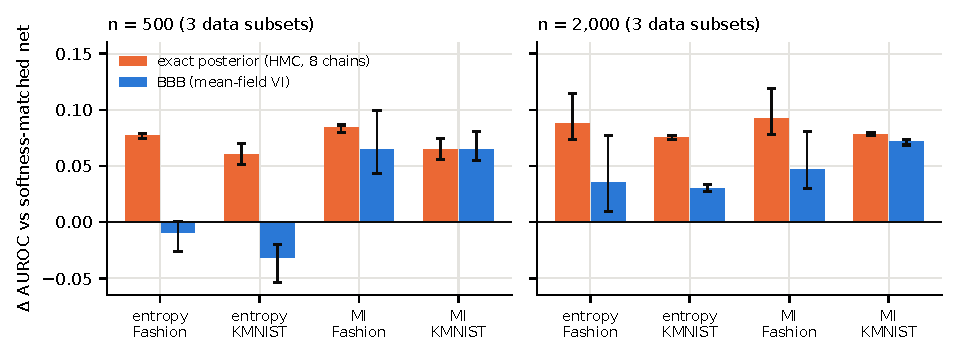
\includegraphics[width=0.85\linewidth]{../figures/E20_hmc.pdf}
\caption{OOD advantage over the softness-matched network for the exact
posterior (HMC) and BBB under the same $\mathcal N(0,0.3^2)$ prior: mean over
three data subsets, bars show the range (E20, E20b).}
\label{fig:hmc}
\end{figure}

\paragraph{Controls for the prior and the sample count.} The softness-matched
network has no prior, while HMC and BBB use $\mathcal N(0,0.3^2)$. A pre-registered
control (E23; Table~\ref{tab:hmc}) trained MAP networks and 5-member MAP
ensembles under the same prior on the same subsets: the ensemble's advantage
($\Delta_K$ $+0.024$ and $\Delta_F$ $+0.033$ at $n=2{,}000$, negative at $n=500$) is
below HMC's on every subset at both $n$, so HMC's advantage comes from posterior
averaging, not from the prior plus ensembling. Evaluating BBB with 800
posterior samples, as many as HMC, changes its numbers by at most 0.01 at
$n=2{,}000$ but raises its entropy-based $\Delta$ by about 0.03 at $n=500$ (to
$+0.000$ and $+0.012$); 50 samples, used for BBB throughout, understate its
entropy-based advantage at small $n$, while its MI-based $\Delta$ barely changes.
With 800 samples BBB's MI-based $\Delta_K$ at $n=2{,}000$ is $+0.077$, against
HMC's $+0.078$.

\paragraph{Checks.} On the first subset, a sampler self-test held:
$\mathbb E[\theta\cdot\nabla U]/d$, which must equal 1 at stationarity, was
0.998--1.002 in every chain. Every single chain shows the advantage
($\Delta_K$ $+0.064$ to $+0.073$), so it is not diversity between chains, and a
single posterior draw is poor (accuracy 0.72 and 0.83), so it comes from
averaging. Part of it comes from HMC's higher accuracy: restricted to test
images that both HMC and the plain network classify correctly, $\Delta$ is
$+0.054$ to $+0.099$. An independent code review of the sampler and analysis
found no error affecting these conclusions (Appendix~\ref{app:hmc}).

\section{BBB gets there by a different route}\label{sec:route}
\paragraph{The exact posterior's information is in correlations.} We had
predicted that the exact posterior would be less ``overpruned'' than BBB; it
is the opposite (E20: 0\% of hidden weights with $|\text{mean}|>\text{std}$
within a chain, against 0.4--1.0\% for BBB). Follow-up analyses (exploratory)
show why. Each weight's marginal under the exact posterior is the prior: the
within-chain standard deviation is 0.299--0.300 in every layer (prior 0.3) and
$|\text{mean}|$ is about 0.02, the sampling error of a mean of 100 draws.
Drawing every weight independently from its HMC marginal gives chance
accuracy (0.09). All of the exact posterior's information is in correlations
between weights, which a mean-field family cannot hold. This is expected for
a model with 89{,}610 parameters and at most 2{,}000 training points, since the
data constrain only a small subspace; we report it as a confirmation that
per-weight summaries cannot distinguish BBB from the exact posterior, not as
a discovery. (The median per-weight lag-1 autocorrelation between kept
samples was $-0.01$, so 100 samples per chain are close to independent.)

\paragraph{BBB's information is in a few precise means.} Long-trained BBB
under $\mathcal N(0,1)$ is overpruned in the sense of
\citet{trippe2018overpruning} (E16, Figure~\ref{fig:prune} in
Appendix~\ref{app:prune}): the median hidden-layer $\sigma$ is 0.71--0.84 and only
1.2--4.5\% of hidden weights have $|\mu|>\sigma$. A pre-registered swap test
shows that both halves of this pairing matter: BBB's variances on the means of
a step-matched plain network give 13--15\% accuracy, and shuffling BBB's
variances within each layer turns the OOD advantage negative ($-0.16$ to
$-0.32$).

\paragraph{A first-layer noise-to-signal ratio, and its limits.}
For an input $x$, the first layer's mean pre-activation is
$m_j=\sum_i\mu_{ij}x_i+\mu_{b_j}$ and the variance posterior noise adds to it is
$v_j=\sum_i\sigma_{ij}^2x_i^2+\sigma_{b_j}^2$. Their ratio
\begin{equation}
R_1(x)=\frac{\sum_j v_j}{\sum_j m_j^2}
\label{eq:r1}
\end{equation}
measures how much noise an input routes through the first layer relative to
the signal it produces. Found in an exploratory analysis (E17) and confirmed
in a separate pre-registered test on ten freshly trained BBB networks and two
OOD sets never used before, grayscale CIFAR-10 and SVHN (E18,
Figure~\ref{fig:r1}), $R_1$ reached AUROC 0.960--0.991 on all four far-OOD
sets, within 0.003--0.019 of BBB's 50-sample mutual information, and
correlated with BBB's per-image MI (Spearman 0.71--0.83). But on these far-OOD
sets, where everything is near the ceiling, a pre-registered comparison with
input-only statistics (E23) shows that this does not single out a mechanism:
the pixel rule of \S\ref{sec:control} correlates with BBB's per-image MI at
least as well as $R_1$ does ($|\rho|$ 0.77--0.87 against 0.71--0.83), so we
cannot claim that $R_1$ explains BBB's far-OOD signal better than where the
ink is. (Resetting those pixels does not change BBB's advantage, so BBB does
not depend on them; they are correlated with what it detects.) $R_1$ does carry
information beyond input statistics on near-OOD rotated digits, where it
reaches AUROC 0.86--0.88 while the image's total ink, its ink count and the
pixel rule are at chance (0.50--0.55); there BBB's own MI is better still
(0.950 against 0.863 at $n=10{,}000$), so deeper layers add information.
Computed from the exact posterior's per-weight moments instead, $R_1$
separates OOD inputs only weakly (0.69--0.88): it describes BBB's mean-field
solution, not the exact posterior. $R_1$ is a first-layer instance of the
moment propagation used in the local reparameterisation trick
\citep{kingma2015variational} and in sampling-free variational inference
\citep{wu2019deterministic,haussmann2019sampling,postels2019sampling}, and a
cheap sampling-free score for a trained BBB network; we do not claim it as a
full account of BBB's OOD behaviour.

\begin{figure}[!htb]
\centering
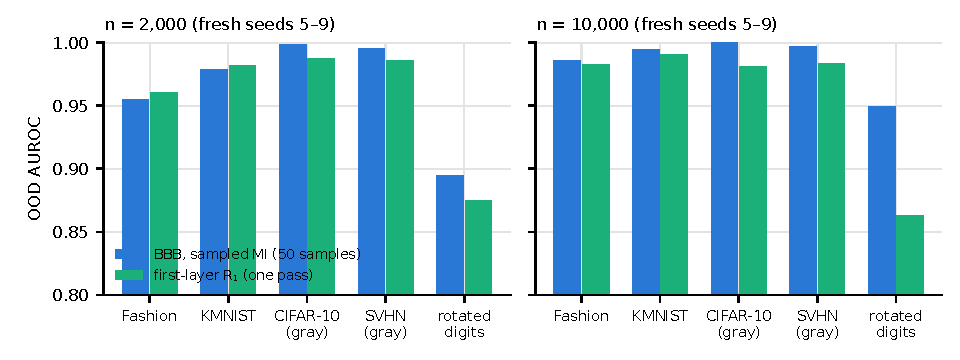
\includegraphics[width=0.85\linewidth]{../figures/E18_r1.pdf}
\caption{OOD AUROC of BBB's sampled mutual information and of the analytic
first-layer ratio $R_1$ (Eq.~\ref{eq:r1}) on freshly trained models (mean of 5
seeds; E18). CIFAR-10 and SVHN were not used anywhere else in the study.}
\label{fig:r1}
\end{figure}

\paragraph{IVON in this light.} IVON's per-weight standard deviations
(0.04--0.17 under $\mathcal N(0,1)$) are far below the spread of exact-posterior
samples, which sits at the prior scale under $\mathcal N(0,0.3^2)$ and had
already reached $\approx0.85$ in the unconverged $\mathcal N(0,1)$ chains. Its
data-scaled variances are therefore not closer to the exact marginals than
BBB's; what BBB shares with the exact posterior is not its marginals but the
size of its epistemic signal.

\section{Related work}
\paragraph{Softness, temperature and OOD baselines.} Temperature scaling
\citep{guo2017calibration} and its role in OOD detection
\citep{liang2018enhancing} motivate the control; \citet{ovadia2019can} include
temperature-scaled baselines and find ensembles strongest under shift,
\citet{ashukha2020pitfalls} argue for comparing uncertainty methods after
temperature scaling, and \citet{abe2022deep} find that ensembles' OOD gains are
largely explained by their in-distribution performance. Our control extends
these to a per-method entropy match for OOD detection. The deterministic
detectors in Table~\ref{tab:controls} are the maximum softmax probability
\citep{hendrycks2017baseline}, the energy score \citep{liu2020energy}, a
Mahalanobis detector \citep{lee2018simple} and deep nearest neighbours
\citep{sun2022knn}; feature-density methods such as DDU
\citep{mukhoti2023ddu} are a stronger deterministic family we did not test.

\paragraph{Mean-field VI and its variances.} \citet{trippe2018overpruning}
describe overpruning; \citet{farquhar2020liberty} argue that deep mean-field
networks can be expressive enough in practice; \citet{coker2022wide} prove that the optimal mean-field
predictive approaches the prior predictive as width grows, consistent with
the drift in \S\ref{sec:clock}; \citet{foong2020expressiveness} show what
mean-field approximations cannot represent; \citet{odgers2026gaussian} show
that mean-field VI can overestimate in-distribution predictive variance.
\citet{unlu2020variational} and \citet{nishida2022adamb} observe unconverged or
growing variance parameters under standard optimizers; we derive the
$N$-independent clock behind this growth and link it to OOD detection.
Natural-gradient methods such as Vadam \citep{khan2018fast}, VOGN
\citep{osawa2019practical} and IVON
\citep{shen2024variational} tie the variances to $N$ and the curvature by
construction.

\paragraph{Exact posteriors and priors.} \citet{izmailov2021what} run
full-batch HMC on much larger networks and find that the exact posterior
predicts well and differs from mean-field VI; we find the same split for OOD
detection at small scale, and that an $\mathcal N(0,1)$ prior makes HMC far
harder than a prior of scale 0.3. \citet{izmailov2021dangers} show that
weights on always-zero pixels keep their prior under HMC and hurt
accuracy under covariate shift, and \citet{kristiadi2020being} show that a
Bayesian last layer reduces overconfidence far from the data, which our
last-layer Laplace results do not reproduce for these OOD sets.
\citet{henning2021bayesian} argue that whether
exact posteriors are good OOD detectors depends on the prior and
architecture; we give one setting where the exact posterior beats a
softness-matched network. \citet{fortuin2022priors} show that isotropic
Gaussian priors are often poor choices, \citet{wenzel2020good} that tempered
posteriors can predict better than the Bayes posterior, and
\citet{depeweg2018decomposition} and \citet{wimmer2023quantifying} discuss the
entropy/mutual-information decomposition our two scores rest on.
\citet{raina2025ood} report Bayesian advantages for OOD detection from small
training sets; our results suggest checking training length and softness
before attributing such gains to the posterior.

\section{Limitations}\label{sec:limits}
\paragraph{Scale and data.} All positive results come from small MLPs on
MNIST-family data (MNIST or Fashion-MNIST as in-distribution), on far-OOD pairs
that a model-free pixel rule nearly solves; on a held-out-class split the
advantage largely disappears. On CIFAR-10 with small, underfit models (a CNN and the
same MLP, 37--68\% accuracy, no augmentation) no comparable advantage
appeared (Appendix~\ref{app:cifar}); this says little about well-trained
networks, and whether the clock and the advantage carry over to modern
architectures is open.
\paragraph{Exact posterior.} HMC converged only under the $\mathcal N(0,0.3^2)$
prior, at width 100, on three data subsets per $n$; under BBB's default
$\mathcal N(0,1)$ prior it did not mix, so the comparison with the exact
posterior does not cover the setting of most other experiments. There is one
HMC run and one BBB model per subset, the $\hat R$ used is not
rank-normalised, and at $n=2{,}000$ the potential drifted slightly between the
halves of sampling (2.2 standard errors).
\paragraph{Design.} Only three prior scales were tried, at one training-set
size; the dynamics runs use a constant learning rate and 3 seeds, the
fixed-budget runs a cosine schedule; the clock was tested with Adam and SGD on
one architecture, with timings resolved to 1{,}000-step checkpoints; all
methods use default hyperparameters without per-method tuning, except IVON's
learning rate and initial Hessian (chosen once by validation NLL); most
comparisons use 5 seeds (3 for the dynamics); and the pre-registration records
are self-attested.

\section{Conclusion}
For Bayes by Backprop on small MLPs and far-OOD MNIST-family benchmarks,
``knowing what it doesn't know'' is not a fixed property of the method: on
MNIST it is set by optimizer time. Under Adam the posterior
variances grow on a learning-rate $\times$ steps clock, almost regardless of
the amount of data, and the OOD advantage over a softness-matched network
switches on with them; where the variances stay small, as under SGD with more
data, there is none. The advantage is not only an artefact of mean-field VI:
under a prior where it can be sampled, the HMC posterior has an advantage
over the softness-matched network, and on KMNIST it is the same size as BBB's
mutual-information signal. But BBB reaches that signal
by a structurally different solution, a few precise means with prior-scale
noise elsewhere, rather than by approximating the exact posterior's marginals.
Comparisons of Bayesian and deterministic OOD detectors should report the
optimizer, learning rate and training budget, the uncertainty score, and a
softness-matched baseline.

\subsubsection*{Broader Impact Statement}
This is a methodological study of uncertainty estimates on public image
benchmarks (MNIST, Fashion-MNIST, KMNIST, CIFAR-10, CIFAR-100, SVHN); it
involves no human subjects and no personal data. Its main societal relevance
is a caution: OOD detection is used to decide when a model's prediction should
not be trusted, and our results show that a Bayesian network's apparent OOD
advantage can depend on the training run, can be matched or exceeded by simple
baselines, and can vanish on near-OOD inputs. Over-reading such advantages could
lead to unwarranted trust in deployed systems; we mitigate this by reporting
softness-matched and step-matched baselines, a near-OOD split and all falsified
predictions, and by recommending that these be reported routinely. All
experiments ran on two consumer GPUs; the method itself poses no apparent
risk of misuse.

\paragraph{Reproducibility.} Code, every command, and every pre-registered
protocol with its result are provided as anonymised supplementary material.

\bibliography{refs}
\bibliographystyle{tmlr}

\appendix
\section{KL scaling}\label{app:kl}
Dividing the KL term in Eq.~\ref{eq:elbo} by the number of mini-batches
instead of by $N$ is an easy slip when the cross-entropy is averaged per
batch. It over-weights the KL term by $N/\lceil N/B\rceil\approx B$ (62.5$\times$
at $N=2{,}000$, $B=64$). In a 3-seed pilot it cost BBB 3.2 points of accuracy
(0.904 vs 0.936) and raised ECE from 0.022 to 0.185. On accuracy, correctly
scaled BBB beats a MAP network trained with the same prior and budget by 1.1
points at $n=500$ and 0.5 points at $n=2{,}000$ (9/10 and 10/10 seeds), and loses by
0.5 points at $n=10{,}000$ (E3).

\section{Always-background pixels}\label{app:pixels}
On average 192, 148 and 104 pixels are constant (always background) across a
training subset at $n=500$, $2{,}000$ and $10{,}000$. Flagging any image with ink
on such a pixel separates MNIST from Fashion-MNIST and KMNIST with AUROC
0.967--1.000 over 15 training subsets (means 0.990--1.000). Resetting those
pixels to background in the OOD images leaves every method's AUROC and
$\Delta$ essentially unchanged (BBB at $n=10{,}000$: $+0.057\to+0.055$ and
$+0.070\to+0.070$), and the growth of $\sigma$ is global rather than
concentrated on those pixels (ratio 1.0--1.24).

\section{Which layers' noise matters}\label{app:layers}
Taking BBB models trained for 23{,}550 steps, we switched posterior noise off
layer by layer (E6b). Noise in the first and second layers together keeps
72--82\% of $\Delta$; noise in any single layer keeps essentially none (first
layer: 16\% on Fashion-MNIST, $-26\%$ on KMNIST), and the posterior-mean network
on its own is a worse OOD detector than the DNN. Noise in the last layer
alone does not reproduce the advantage in this model, which may explain why
last-layer Laplace does poorly in Table~\ref{tab:grid}.

\section{BBB's overpruned posterior}\label{app:prune}
\begin{figure}[!htb]
\centering
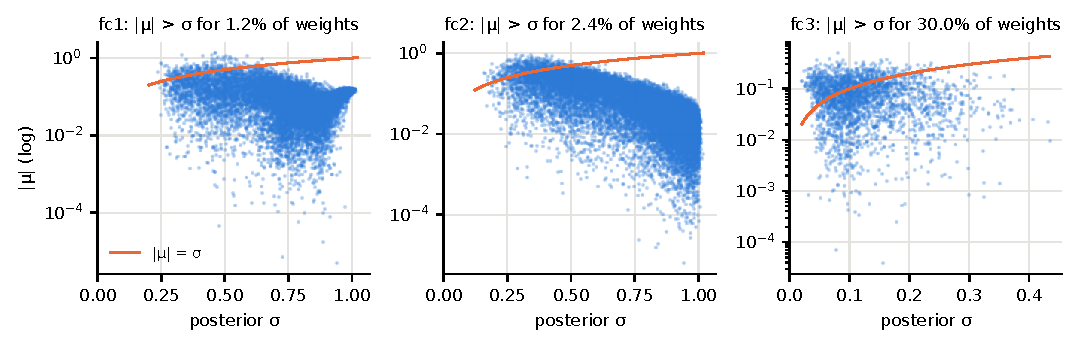
\includegraphics[width=\linewidth]{../figures/E16_overpruning.pdf}
\caption{Posterior mean magnitude against posterior $\sigma$ for every weight of a
BBB network trained for 23{,}550 steps ($n=2{,}000$, seed 0; 20{,}000 weights
sampled per layer; E16). In the second layer $|\mu|$ and $\sigma$ are strongly
anti-correlated ($-0.64$ to $-0.72$), and the last layer is nearly
deterministic.}
\label{fig:prune}
\end{figure}

\section{Choosing when to stop}\label{app:stop}
Minimum held-out NLL stops at 1{,}000--3{,}000 steps, before the advantage
appears; minimum $-$ELBO stops at the end of training. A rule that needs no
real OOD data, picking the checkpoint that best separates validation images
from three synthetic outlier sets (uniform noise, flipped digits,
pixel-permuted digits) by MI, reaches 74\% of the best achievable
entropy-based advantage (an optimistic oracle over 40 checkpoints), but simply
stopping at a fixed 8{,}000 steps reaches 72\% (Table~\ref{tab:select}; 12
runs, $n\in\{500, 2{,}000, 10{,}000\}$; E9). Scoring the last checkpoint by MI
instead of entropy, with no selection at all, does as well ($+0.049$).

\begin{table}[!htb]
\centering\small
\caption{Stopping rules ($\bar\Delta$ = mean of Fashion-MNIST and KMNIST
entropy-based $\Delta$ at the chosen checkpoint; 12 runs; E9).}
\label{tab:select}
\begin{tabular}{lccc}
\toprule
rule & mean step & $\bar\Delta$ (entropy) & fraction of oracle \\
\midrule
oracle (uses real OOD; optimistic) & 10{,}917 & $+0.067$ & 1.00 \\
synthetic-outlier proxies (MI) & 10{,}417 & $+0.049$ & 0.74 \\
fixed stop at 8{,}000 steps & 8{,}000 & $+0.048$ & 0.72 \\
fixed stop at 10{,}000 steps & 10{,}000 & $+0.047$ & 0.71 \\
minimum $-$ELBO & 39{,}417 & $+0.034$ & 0.51 \\
minimum validation NLL & 2{,}250 & $-0.032$ & $-0.48$ \\
\bottomrule
\end{tabular}
\end{table}

\section{CIFAR-10}\label{app:cifar}
We repeated the dynamics experiment on CIFAR-10 ($n=10{,}000$, no augmentation)
with a small CNN (three $3\times3$ convolutional layers of 32, 64 and 128
channels, then 256 and 10 units), every layer Bayesian, with SVHN and
CIFAR-100 as OOD sets (E7). No comparable advantage appeared
(Figure~\ref{fig:cifar}): BBB's peak $\Delta$ on SVHN was $-0.044$, $+0.006$ and
$-0.056$ in the three seeds, and on CIFAR-100 at most $+0.031$, early in
training. Even a 5-member deep ensemble lost to a single softness-matched DNN
on SVHN (AUROC 0.727--0.740 vs 0.759--0.807). The drift towards the prior did
replicate: the fully connected layer's $\sigma$ reached 0.996 and accuracy fell
from 0.67--0.68 to 0.61--0.63. The MNIST study's MLP on flattened CIFAR-10
images (E7b; 38\% and 46\% deterministic accuracy at $n=2{,}000$ and $10{,}000$)
also showed no advantage on SVHN (peak $\Delta$ $-0.031$ to $+0.030$); its
CIFAR-100 gains ($+0.030$ to $+0.046$ early in training) were similar to the
CNN's, and larger ``gains'' appeared only after collapse to near-chance
accuracy. These models are small and underfit, so this negative result says
little about well-trained networks.

\begin{figure}[!htb]
\centering
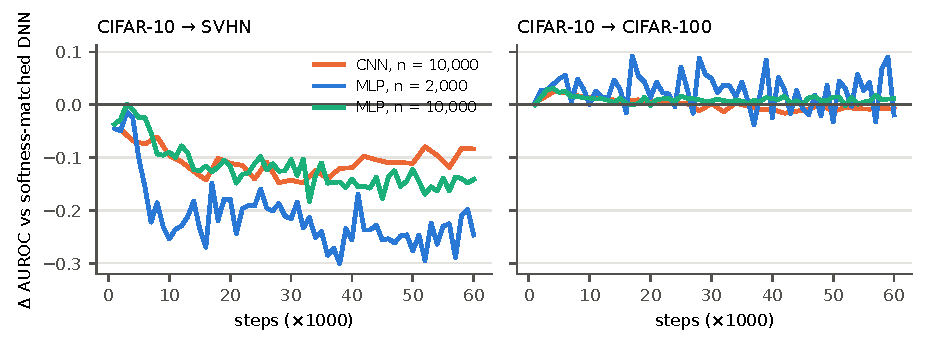
\includegraphics[width=0.85\linewidth]{../figures/paper_cifar.pdf}
\caption{BBB against its softness-matched network on CIFAR-10 over training
(mean of 3 seeds per curve; E7, E7b).}
\label{fig:cifar}
\end{figure}

\section{HMC details}\label{app:hmc}
\paragraph{Sampler.} Full-batch HMC in PyTorch, with all chains of a run
batched in one process (the per-chain implementation was limited by Python
overhead, not by the GPU). Each chain starts from its own MAP estimate (3{,}000
full-batch Adam steps from a different random initialisation), uses an
identity mass matrix, adapts its step size by dual averaging towards 0.8
acceptance over 500 warm-up iterations and then freezes it (with $\pm10\%$
jitter), and uses $L=\lceil 0.471/\text{median step}\rceil$ leapfrog steps
(360--430 at $n=500$, 702--856 at $n=2{,}000$). Every tenth of 1{,}000 sampling
iterations is kept. A run takes about 25 minutes ($n=500$) and 55 minutes
($n=2{,}000$) on one RTX 3090.

\paragraph{Convergence.} Split-$\hat R$ over the 8 chains on the predicted
probability of the true class for 1{,}000 fixed test images; a run counts as
converged if the 90th percentile is below 1.1 (decided before running). The
mean potential changed by $-1.9$ and $+11.6$ between the halves of sampling on
the first subset (batch-means standard errors 5.5 and 5.3). The self-test
$\mathbb E[\theta\cdot\nabla U]=d$ holds for any differentiable target at
stationarity; a wrong gradient, kinetic energy or acceptance step would
violate it.

\paragraph{The $\mathcal N(0,1)$ attempt (E19).} 4 chains, 300 leapfrog steps,
Robbins--Monro step-size adaptation over 1{,}500 warm-up iterations, 1{,}000
sampling iterations. The adapted step size (2.3--5.4$\times10^{-5}$) moved each
chain only $\sim$0.01 per iteration, the potential was still rising during
sampling, and the spread of weight means across chains was 6--8$\times$ the
within-chain standard deviation. Under $\mathcal N(0,1)$ the stable step
shrinks as trajectories lengthen, so longer runs would not fix this at an
affordable cost; a diagonal mass matrix estimated in Stan-style windows
reduced the step size further, and a width-20 network gave a step of
$10^{-5}$ at 3{,}000 leapfrog steps.

\paragraph{Independent code review.} A separate AI agent (a large language
model run independently of the analysis, with read-only access to the code and
results) audited the sampler and analysis code (kinetic energy and acceptance, state after accept/reject,
state-independent step size and trajectory length, exclusion of warm-up
samples, $\hat R$ axes, validation-only temperature fit, identical data
subsets for HMC, BBB and the plain network) and recomputed $\Delta$
independently; it found no error affecting the conclusions. Its suggestions
(accuracy-matched $\Delta$, drift standard errors, seed spread) are reported
above.

\section{Pre-registered predictions and outcomes}\label{app:ledger}
Each protocol was written before its runs: committed to version control for
E1--E9 and, for E10--E23, with a SHA-256 hash recorded before launch
(self-attested, not independently timestamped). Of the 87 entries below, 39
were confirmed, 31 falsified, 13 had mixed outcomes, 3 had no outcome and 1
was a decision rule. (E5's first prediction held by construction and is
omitted.) The falsified ones are what moved the study from ``is the
advantage just softness?'' to the training-path account.

{\small
\begin{longtable}{p{0.9cm}p{8.6cm}p{4.6cm}}
\toprule
exp. & prediction & outcome \\
\midrule
\endfirsthead
\toprule
exp. & prediction & outcome \\
\midrule
\endhead
\bottomrule
\endlastfoot
E1 & P0: new pipeline reproduces old numbers ($\pm0.02$ acc, $\pm0.03$ AUROC) & acc/ECE yes; AUROC off by 0.035 \\
E1 & P1: correct KL weight raises BBB accuracy & confirmed \\
E1 & P2: BBB within 0.02 AUROC of softness-matched DNN & falsified (Fashion) \\
E2 & P1: BBB never beats the control & falsified ($n=10{,}000$) \\
E2 & P2: ensembles beat the control & confirmed \\
E2 & P3: MC dropout and Laplace within 0.02 of the control & dropout yes; Laplace falsified \\
E2 & P4: larger KL weight lowers accuracy, raises KMNIST MI-AUROC & confirmed \\
E3 & P1: BBB and budget-matched MAP equally accurate ($<0.005$) & falsified (narrowly) \\
E3 & P2: BBB never beats softness-matched MAP & falsified ($n=10{,}000$) \\
E4 & P1: the gain follows optimizer steps, not $n$ & confirmed \\
E4 & P2: dead-pixel weights have $>5\times$ the $\sigma$ of live ones & falsified \\
E4 & P3: $n=500$ with long training shows the gain & confirmed \\
E5 & P2: removing dead-pixel ink halves BBB's gain & falsified \\
E5 & P3: removing it shrinks the ensemble's gain & falsified \\
E5 & P4: the DNN's AUROC drops less than BBB's when the ink is removed & falsified (neither drops) \\
E6 & P1: $\Delta$ rises with $\sigma$ & falsified (peaks, then falls) \\
E6 & P2: $\Delta$ plateaus & falsified (transient) \\
E6 & P3: larger $\sigma_0$ reaches the gain sooner & falsified ($\sigma_0\ge0.31$ never learns) \\
E6 & P4: ELBO still improving at 4{,}800 steps & confirmed \\
E6b & P1: first-layer noise alone keeps $\ge70\%$ & falsified \\
E6b & P2: last-layer noise alone keeps $<30\%$ & confirmed \\
E9 & P1: combined proxies reach $\ge70\%$ of oracle; NLL $\le20\%$ & confirmed, but a fixed 8k-step stop does as well \\
E9 & P2: one proxy alone reaches $\ge70\%$ & falsified (67\%) \\
E9 & P3: peak step rises with $n$ & confirmed by mean; not robust \\
E7 & P1: window on SVHN with a CNN & falsified \\
E7 & P2: window closes & no outcome (no window) \\
E7 & P3: proxy selection beats NLL & falsified \\
E7 & P4: ensemble beats the control on SVHN & falsified \\
E7b & rule: architecture vs data & ``architecture'' by the rule; weak \\
E10 & P1: time to $\sigma=0.3$ $\times$ learning rate constant ($\pm30\%$) & confirmed \\
E10 & P2: under Adam, $n$ changes that time by $\le25\%$ & confirmed \\
E10 & P3: under SGD, $\sigma$ grows $\ge3\times$ faster at $n=500$ than $10{,}000$ & confirmed (39$\times$) \\
E10 & P4: onset of the OOD advantage follows the same clock ($\pm40\%$) & confirmed \\
E11 & P1: a tighter prior improves final accuracy & falsified \\
E11 & P2: a tighter prior keeps the entropy advantage to the end & $\sigma_p=0.3$ yes; 0.1 no \\
E11 & P3: MI advantage survives $\sigma_p\in\{0.1, 0.3\}$ (kill test) & confirmed \\
E12 & P1: weight noise stays $\ge0.02$ below BBB & confirmed \\
E12 & P2: step-matched softened network stays $\ge0.04$ below BBB & confirmed (narrowly) \\
E12 & P3: step-matched ensemble stays below BBB & confirmed \\
E12 & P4: feature detectors $\ge0.95$ and within 0.03 of BBB & kNN yes; Mahalanobis no \\
E13 & P1: without joint clipping, SGD $\sigma$ still grows $\ge3\times$ faster at $n=500$ & confirmed (53$\times$, one $n=500$ seed past 20k) \\
E13 & P2: $\rho$ learning rate $\propto N$ aligns the clocks across $n$ & falsified as scored (1 run diverged first; 2 crossed just before diverging) \\
E13 & P3: with that scaling, the OOD advantage appears at $n=10{,}000$ & falsified (runs diverged first) \\
E14 & P1: IVON's $\sigma$ is $\ge2\times$ larger at $n=500$ than $10{,}000$ & confirmed (4.41$\times$) \\
E14 & P2: IVON's $\sigma\le0.3$ at $n\ge2{,}000$ & confirmed \\
E14 & P3: IVON shows no transient & $n\ge2{,}000$ yes; $n=500$ no \\
E14 & P4: IVON's advantage below BBB's but $\ge0$ & below BBB yes; $\ge0$ no \\
E14 & P5: IVON accuracy within 0.01 of the plain network & $n\ge2{,}000$ yes; $n=500$ no \\
E15 & P1: tempering raises IVON's $\sigma$ & confirmed \\
E15 & P2: at $k=100$, IVON gains an advantage $\ge0.03$ & falsified (collapse) \\
E15 & P3: at $k=10$, accuracy within 0.02 & $n=10{,}000$ yes; $n=2{,}000$ no \\
E16 & P1: BBB's $\sigma$ on plain-network means collapses accuracy & confirmed \\
E16 & P2: that swap loses $\ge0.05$ of the advantage & confirmed \\
E16 & P3: shuffling $\sigma$ within layers keeps $\ge80\%$ & falsified \\
E17 & P1: second-layer ratio $R_2$ separates OOD (AUROC $\ge0.90$) & falsified \\
E17 & P2: $R_2$ correlates with MI ($\ge0.6$) & falsified \\
E17 & P3: $R_2$ separates better than $R_1$ & falsified \\
E18 & P1: $R_1$ AUROC $\ge0.90$ on four far-OOD sets (fresh models) & confirmed \\
E18 & P2: $R_1$ within 0.03 of BBB's MI & confirmed \\
E18 & P3: Spearman($R_1$, MI) $\ge0.6$ & confirmed \\
E18 & P4: $R_1$ within 0.05 of MI on rotated digits & $n=2{,}000$ yes; $n=10{,}000$ no \\
E19 & P1: decision rule on HMC's $\Delta$ (exact posterior) & no outcome: chains did not converge ($\hat R$ 90th pct.\ 2.5--2.8) \\
E19 & P2: HMC less overpruned than BBB ($\ge2\times$) & no outcome: within-chain spread reflects poor mixing \\
E19 & P3: HMC accuracy $\ge$ BBB at $n\in\{500,2000\}$ & falsified (0.899 vs 0.920; 0.833 vs 0.881), exploratory \\
E20 & P1: decision rule on HMC's $\Delta$ under $\mathcal N(0,0.3^2)$ (converged) & decision: advantage at both $n$ \\
E20 & P2: HMC less overpruned than BBB ($\ge2\times$) & falsified (0\% vs 0.4--1.0\%) \\
E20 & P3: HMC accuracy $\ge$ BBB & confirmed (0.890 vs 0.798; 0.929 vs 0.909) \\
E20 & P4: HMC and BBB MI $\Delta_K$ within 0.03 & confirmed (0.006 at both $n$) \\
E20b & Q1: HMC $\Delta_K,\Delta_F\ge+0.03$ on every subset & confirmed (6/6 runs) \\
E20b & Q2: mean $|$MI $\Delta_K$ HMC $-$ BBB$|\le0.03$ & confirmed (0.006, 0.007) \\
E20b & Q3: HMC accuracy $\ge$ BBB on every subset & confirmed (6/6) \\
E20b & Q4: HMC entropy $\Delta_K$ exceeds BBB's by $\ge0.02$ & confirmed ($+0.092$, $+0.045$) \\
E21 & P1: Fashion-MNIST ID, standard-budget BBB $\Delta\le+0.02$ & falsified ($+0.080$, $+0.066$) \\
E21 & P2: long-trained BBB $\Delta\ge+0.03$, $\ge4/5$ seeds, both OOD sets & confirmed ($+0.136$, $+0.082$; 5/5) \\
E21 & P3: long BBB beats step-matched DNN and ensemble ($\ge4/5$ seeds) & DNN yes (5/5, 5/5); ensemble MNIST 5/5, KMNIST 2/5 \\
E21 & P4: $n=10{,}000$ BBB $\Delta\ge+0.03$ & confirmed ($+0.160$, $+0.206$) \\
E21 & P5: long BBB MI $\Delta\ge+0.03$ on both OOD sets & KMNIST yes ($+0.205$); MNIST no ($+0.015$) \\
E22 & P1: digits 0--4 ID; long BBB $\Delta\ge+0.02$ on held-out digits 5--9 & falsified ($+0.011$, 4/5) \\
E22 & P2: held-out-digit $\Delta$ below far-OOD $\Delta$ & confirmed ($+0.011$ vs $+0.041$) \\
E22 & P3: long BBB beats step-matched DNN and ensemble on held-out digits & falsified (3/5, 1/5) \\
E22 & P4: pixel rule AUROC on held-out digits $\le0.80$ & confirmed (0.569) \\
E22 & P5: standard-budget BBB held-out $\Delta\le+0.02$ & falsified ($+0.023$) \\
E23 & P1: HMC $\Delta$ exceeds a MAP ensemble's under the same prior, every subset & confirmed (3/3 at both $n$) \\
E23 & P2: single MAP under the same prior, mean $\Delta_K\le+0.02$ & confirmed ($-0.015$, $+0.017$) \\
E23 & P3: BBB with 800 vs 50 samples changes $\Delta$ by $\le0.01$ & $n=2{,}000$ yes; $n=500$ no ($+0.032$) \\
E23 & P4: $R_1$ tracks BBB's MI better than input-only baselines (far OOD) & falsified (pixel rule $|\rho|$ 0.77--0.87 vs 0.71--0.83) \\
E23 & P5: $R_1$ beats input-only baselines on rotated digits & confirmed (0.86--0.88 vs 0.50--0.55) \\
\end{longtable}
}

\end{document}
